\section{Pregled}

\subsection{Arhitektura}
Cijeli sustav je rastavljen u 3 glavna dijela
\begin{itemize}
  \item Transkoder
  \item Server
  \item Klijenti
\end{itemize}
\paragraph{Transkoder}
je zadužen za primanje podataka od kamere i transformiranje istih u format koji je odgovarajuć za najveći broj klijenata, 
te slanje u realnom vremenu na server TCP protokolom.
\paragraph{Server}
je zadužen za autoriziranje klijenata te prosljeđivanje paketa koje prima od Transkodera HTTP protokolom.
\paragraph{Klijenti}
nakon što se autoriziraju sa serverom, preko HTTP-om primaju pakete videa te ih prikazuju korisniku.
\begin{figure}[h]
  \centering
  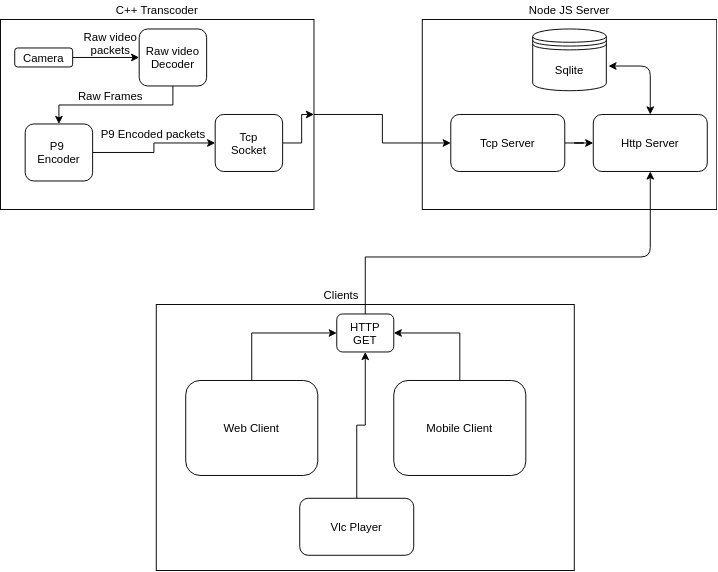
\includegraphics[width=\textwidth]{flow-diagram.png}
  \caption{Flow diagram sustava}
\end{figure}

\clearpage
\subsection{Tehnologije}

\subsubsection{C++}
C++ je odabran za implementaciju transkodera, primarno zato jer su FFMpeg biblioteke napisane u jeziku C sa kojim se C++ vrlo jednostavno integrira ali
i zbog manjka memorije Rasbperry pia.

\subsubsection{Node JS}
Node JS je open-source cross-platform runtime za JavaScript. \\
Omogučuje pisanje serverskog koda u jeziku JavaScript.
\paraBreak
Idealan je za server ovog projekta zbog svog event-driven asinkronog pristupa, operira sa samo jednom dretvom koja nikad ne čeka.
\paraBreak
To postiže koristeći dijeljeni task queue, glavni JavaScript thread samo šalje poslove u task queue i registrira funkciju koja če se izvršit kada taj posao zavrsi, 
task queue zatim kada dođe do tog posla izvrši ga te pozove registriranu funkciju sa rezultatom te nastavi dalje.

\subsubsection{React JS}
React JS je \foreign{open-source} JavaScript biblioteka za izradu web aplikacija.
\paraBreak


\subsubsection{Flutter}
Flutter je \foreign{open-source} framework za izradu cross-platform mobilnih aplikacija.

\clearpage
\subsection{Video}
Video je ništa drugo nego niz slika koje se mijenjaju određenom frekvencijom, u slučaju filmova naj češće 24 slika po sekundi (24 FPS).

\subsubsection{Kontejner}
Kontejner je jedan file koji sadrži sve tokove (\foreign{stream}) kao što su video, audio, titlovi itd.\\
Još sadrži sve metapodatke kao što su rezolucija videa, FPS, autor, kodek itd. Po tim podacima video playeri znaju korektno prikazati sliku i zvuk.

\subsubsection{Kodek}
Problem kod videa je veličina, recimo da imamo video rezolucije 1920 x 1080 koji se vrti na 24 FPS, i da koristimo RGB pixel format
što znači da nam trebaju 3 bajta po pixelu za enkodiranje boje te da traje 30 minuta \\
Veličina takvog videa bila bi \textbf{268.7 GB}
\paraBreak
Upravo iz tog razloga moramo imati kodek.

\subsubsection{Podržanost}
Za živi prijenos postoje 3 naj bolje opcije što se tiče podržanosti

\myparagraph{h264 + rtmp}
H264 je jedan od naj starijih kodeka i kao takav podržan je na skoro svim uređajima.
Nudi dobar balans kvalitete i brzine.
\paraBreak
Rtmp kontejner je jedan od naj korištenijih kontejnera za živi prijenos, jedan od korisnika je Twitch.tv \\
Problem ovog kontejner je sto je vlasnik Adobe i nije besplatan, uz to nije podržan nativno u browserovom HTML5 video elementu.

\myparagraph{h264 + mp4}
U teoriji odlična kombinacija jer je mp4 kontejner podržan virtualno svugdje.
\paraBreak
Nažalost mp4 ne podržava živi prijenos jer mora unaprijed znat točnu duljinu videa što kod živog prijenosa nije moguće. \\
Rješenje je MPEG-DASH (Dynamic Adaptive Streaming over HTTP). Ono razdvoji video u manje cjeline (chunks) sa poznatom veličinom.

\myparagraph{vp8/9 + webm}
Ovu kombinaciju kodeka i kontejnera je implementirao Google, želeći izbjeći troškove licenci za 264/5 kodek. \\
Glavna snaga mu je odlična kompatibilnost sa nativnim HTML 5 video elementom koji je standard u većini preglednika
\paraBreak
Osim toga u usporedbi s puno starijim h264 kodekom, pruža bolju latenciju i kvalitetu slike, pogotovo na nižim \foreign{bit rate} a uz to je
i efikasniji što se tiče resursa.
\paraBreak
Najveći problem mu je Apple koji odbija implementirati ovu kombinaciju u Safariju i IOS operativnom sustavu. \\
Također za razliku od mp4 kontejnera webm nije kodek agnostičan, to jest može se kombinirati samo sa vp8 ili vp9 kodecima.
\paraBreak
Upravo ova kombinacija je odabrana u ovom radu zbog svoje relativne jednostavnosti i dobre podržanosti.

\begin{center}
  \begin{table}[h]
  \begin{tabular}{|c|c|c|c|}
    \hline
      & vp8/9 + webm & h264+mp4/DASH & h264 + mkv \\
    \hline
    Chrome & x & x & - \\
    Firefox & x & x & - \\
    Safari & - & x & - \\
    Edge & vp8 & x & - \\
    IOS (Svi preglednici) & - & x & - \\
    Android (Chrome) & x & x & - \\
    \hline
  \end{tabular}
  \caption{Podržanost kodeka i kontejnera u raznim preglednicima}
\end{table}

\end{center}


\subsubsection{Dekodiranje}
\subsubsection{Enkodiranje}

\clearpage
\subsection{Umreženost}
